\documentclass[11pt,a4paper]{article}

% package importing
%\usepackage[margin=2cm]{geometry}
\usepackage{geometry}
 \geometry{
 a4paper,
 %total={170mm,257mm},
 left=20mm,
 top=20mm,
 right=20mm,
 bottom=20mm,
 }
 		%$$$$$$ fonts settings $$$$$$%
%\usepackage[sc]{mathpazo}  %for palatino font
%\usepackage{eulervm}  %for Euler maths font

		%$$$$$$ package imports $$$$$$%
\usepackage{amsmath}  %for mathematics
\usepackage{titlesec}  %for title spacing only
\usepackage{lipsum}  %random huge text generation
\usepackage{titlesec} %for changing font of titles 
\usepackage{amssymb}  %for real number set symbol
\usepackage{amsthm}  %for mathematics package
\usepackage{mathtools}  %for floor and ceiling
\usepackage{algorithmicx}  %for dynamic algorithm
\usepackage{algorithm}  %algorithm micro
\usepackage{algpseudocode}  %pseudocode commands
\usepackage{wrapfig}  %for wrapping figures around text
\usepackage{multicol}  %for multiple columns floats
\usepackage{enumitem}  %for enumerate numbering
\usepackage{url}   %for writing the url
\usepackage{color}  %for colorred text
\usepackage{tcolorbox}  %for colour box highlighting
\usepackage{listings}  %for code listing

% $$$$$$$$$ new command and theorems self-defined
\theoremstyle{definition}
\newtheorem{theorem}{Theorem}[section]
\newtheorem{corollary}{Corollary}[theorem]
\newtheorem{lemma}[theorem]{Lemma}
\newtheorem*{remark}{Remark}
\newtheorem{definition}{Definition}[section]
\newtheorem{example}{Example}[section]
\newtheorem{notation}{Notation}[section]
\newtheorem{algoalgorithm}{Algorithm}[section]
\newtheorem{method}{Method}[section]

% $$$$$$$$ set general info $$$$$$$
\title{\textsl{National University of Singapore} \\ \textbf{CS2106 Operating System}\\ Second Half Summary Notes}
\author{\textit{Dong Shaocong} A0148008J}

% $$$$$$$$ package parameter setting $$$$$$$$$

% for title spacing {left}{before}{after}  ----------------------------
\titlespacing\section{0.5pt}{10pt plus 2pt minus 2pt}{2pt plus 2pt minus 1pt}
\titlespacing\subsection{0.5pt}{10pt plus 2pt minus 2pt}{2pt plus 2pt minus 1pt}
\titlespacing\subsubsection{0.5pt}{10pt plus 2pt minus 2pt}{2pt plus 2pt minus 1pt}

% for title font specifications  ------------------------------------------
\titleformat{\section}
  {\normalfont\fontsize{16}{16}\bfseries}
  {\thesection}{1em}{}
  
\titleformat{\subsection}
  {\normalfont\fontsize{14}{14}\bfseries}{\thesection}{1em}{}
  
\titleformat{\subsubsection}
  {\normalfont\fontsize{13}{13}\bfseries}{\thesection}{1em}{}

% declare floor and ceiling functions   ------------------------------------------
\DeclarePairedDelimiter\ceil{\lceil}{\rceil}
\DeclarePairedDelimiter\floor{\lfloor}{\rfloor}

% set the numbering of enumerate to numbers------------------------------------------
\setlist[enumerate]{label*=\arabic*.}
%\setlist{nolistsep}
\newenvironment{myitemize}
{ \begin{itemize}
    \setlength{\itemsep}{5pt}
    \setlength{\parskip}{0pt}
    \setlength{\parsep}{0pt}     }
{ \end{itemize}                  } 
\newenvironment{myenumerate}
{ \begin{enumerate}
    \setlength{\itemsep}{5pt}
    \setlength{\parskip}{0pt}
    \setlength{\parsep}{0pt}     }
{ \end{enumerate}                } 

% $$$$$$$$$ math symbols cheatsheet
% Caligraphic letters: $\mathcal{A}$ 
% Mathbb letters: $\mathbb{A}$
% Mathfrak letters: $\mathfrak{A}$ 
% Math Sans serif letters: $\mathsf{A}$ 
% $$$$$ color text commands ------------
\newcommand{\redtt}[1]{{\color{red}\texttt{#1}}}
\newcommand{\bluett}[1]{{\color{blue}\texttt{#1}}}
\newcommand{\browntt}[1]{{\color{brown}\texttt{#1}}}
\newcommand{\bluebf}[1]{{\color{blue} \huge \textbf{#1}}}
\renewcommand{\emph}[2]{\redtt{#1} \bluebf{#2}}
%-------------------------------------------------------

% $$$$$$$$ start of documents $$$$$$$$$
\begin{document}
\maketitle
\section{I/O System}

\begin{definition}{\textbf{I/O Devices}}
	\begin{myitemize}
		\item \textbf{Communication devices}: Input only (mouse, keyboard); output only (display); Input/output (network card)
		\item \textbf{Storage devices}: Input/output (disk, tape); Input only (CD-ROM)
	\end{myitemize}
\end{definition}

\begin{definition}{\textbf{Main tasks of I/O System}}
	\begin{myitemize}
		\item Present \textbf{logical} (abstract) view of devices (\textbf{hide}: details of hardware interface and error handling)
		\item Facilitate \textbf{efficient} use: overlap CPU and I/O
		\item Support \textbf{sharing} of devices: protection when device is shared (disk), scheduling when exclusive access needed (printer)
	\end{myitemize}
\end{definition}

\begin{definition}{\textbf{Block-Oriented Device Interface}}
	\begin{myitemize}
		\item \textbf{Description}: direct access, contiguous blocks, usually fixed block size
		\item \textbf{Operation}:
		\begin{myitemize}
			\item \textbf{Open}: verify device is ready, prepare it for access
			\item \textbf{Read}: Copy a block into main memory 
			\item \textbf{Write}: Copy a portion of main memory to a block
			\item \textbf{Close}: Release the device
			\item \textbf{*Note}: these are lower level than those of the FS 
		\end{myitemize}
		\item \textbf{Application}: Used by File System and Virtual Memory System; Applications typically go through the File System
	\end{myitemize}
\end{definition}

\begin{definition}{\textbf{Stream-Oriented Device Interface}}
	\begin{myitemize}
		\item \textbf{Description}: character-oriented, sequential access
		\item \textbf{Operation}:
		\begin{myitemize}
			\item \textbf{Open}: reserve exclusive access
			\item \textbf{Get}: return next character of input stream
			\item \textbf{Put}: append character to output stream
			\item \textbf{Close}: release exclusive access
			\item \textbf{*Note}: these too are different from those of the FS but some systems try to present a uniform view of files and devices 
		\end{myitemize}
	\end{myitemize}
\end{definition}

\begin{minipage}{0.35\linewidth}
	\begin{definition}{\textbf{I/O Devices - Ouput}}
		\begin{myitemize}
			\item \textbf{Display monitors}: 
			\begin{myitemize}
				\item character or 
graphics oriented
				\item Different data rates: 25 x 80 characters vs 800 x 600 pixels (1B allows 256 colors) Refresh 30-60 times/s for video 
			\end{myitemize}
			\item \textbf{Printers (ink jet, laser)}
			\item \textbf{Interface}:
			\begin{myitemize}
				\item \textbf{write} to controller buffer
				\item \textbf{wait} for completion
				\item handle \textbf{errors}
			\end{myitemize}
		\end{myitemize}
	\end{definition}
\end{minipage}
\begin{minipage}{0.65\linewidth}
	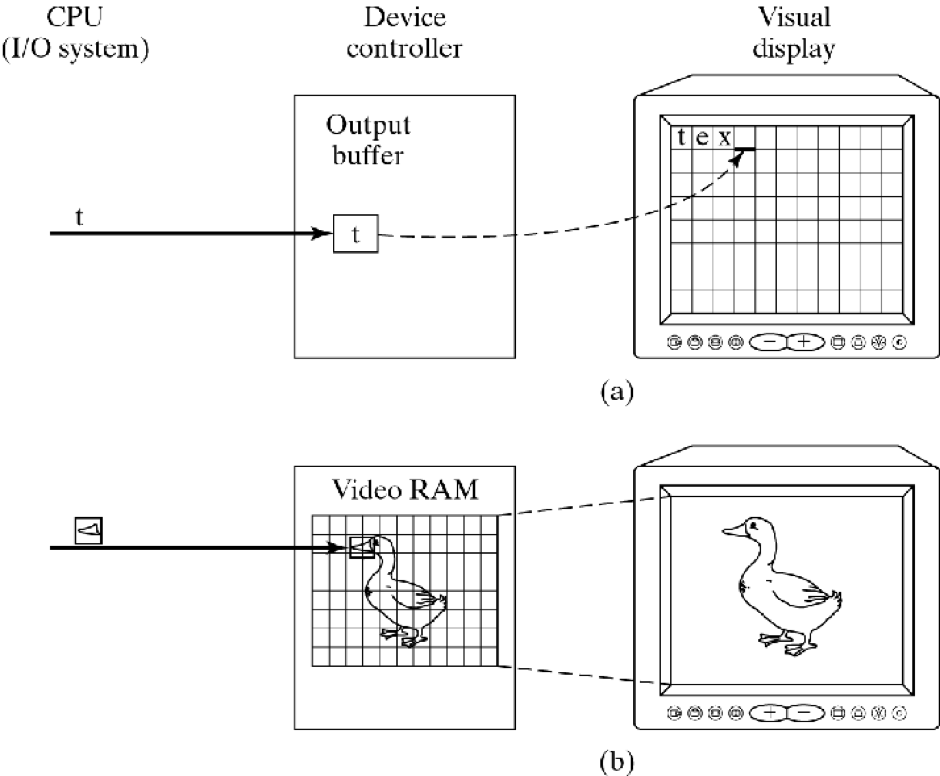
\includegraphics[width=\linewidth]{m3/output}
\end{minipage}

\begin{definition}{\textbf{I/O Devices - Input}}
	Keyboards, pointing devices (mouse, trackball, joystick), scanners. \textbf{Interface}: 
	\begin{myitemize}
		\item device generates interrupt when data is ready
		\item read data from controller buffer
		\item low data rates, not time-critical
	\end{myitemize}
\end{definition}

\begin{definition}{\textbf{I/O Devices - Storage}}

	\begin{minipage}{0.3\linewidth}
		\begin{myitemize}
			\item Surface, tracks/surface, sectors/track, bytes/sector
			\item All sectors numbered sequentially $0..(n-1)$, device controller provides mapping
		\end{myitemize}
	\end{minipage}
	\begin{minipage}{0.7\linewidth}
		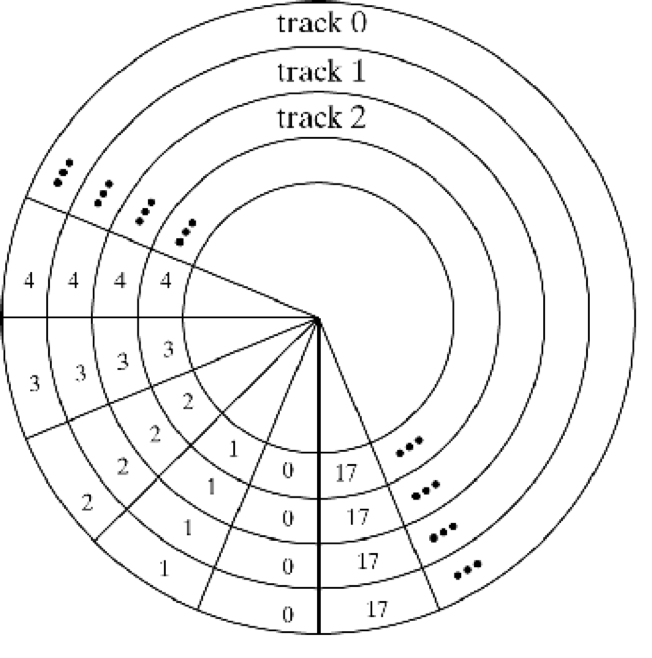
\includegraphics[width=0.5\linewidth]{m3/diskTrackView1}
		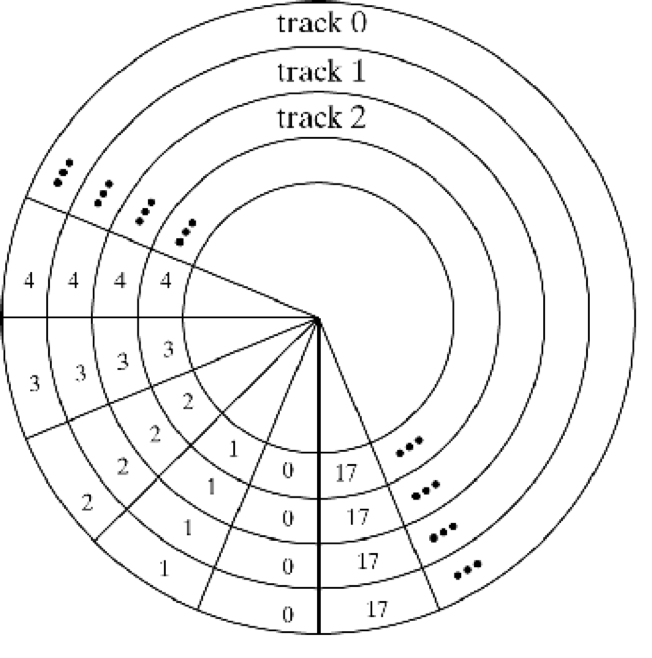
\includegraphics[width=0.5\linewidth]{m3/diskTrackView1}
	\end{minipage}
	
	\begin{minipage}{0.3\linewidth}
		\textbf{Track skew}: account for seek-to-next-track to minimise rotational delay
		
		\[\frac{\text{track to track seek time}}{\text{rotational time per track}} \times \text{sect} \]
		\[\text{ors per track} = \text{offset}\]
		\[\text{Round up the result} \]
	\end{minipage}
	\begin{minipage}{0.7\linewidth}
		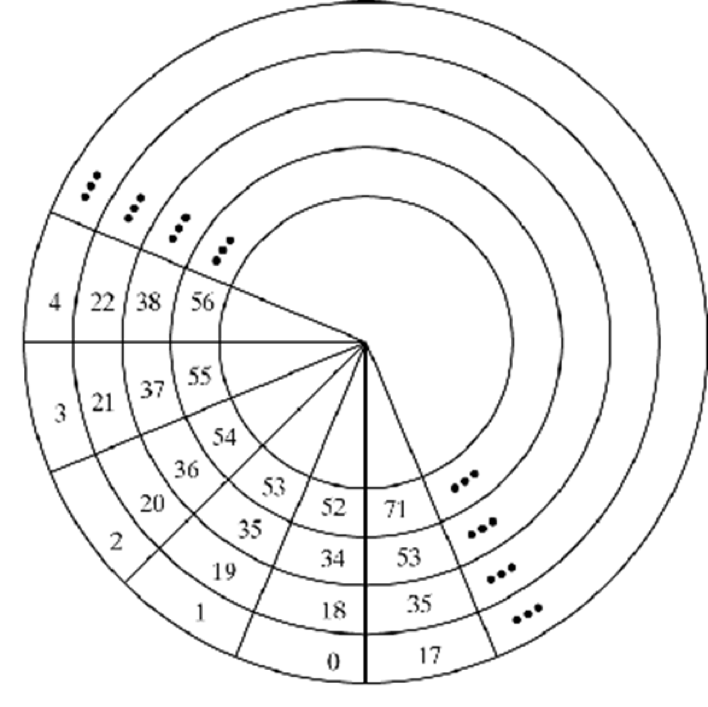
\includegraphics[width=0.5\linewidth]{m3/diskTrackView3}
		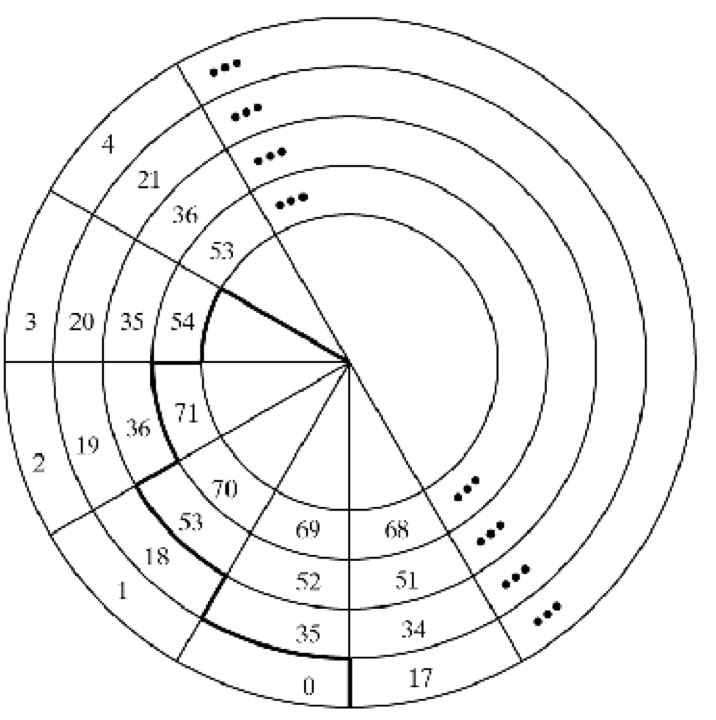
\includegraphics[width=0.5\linewidth]{m3/diskTrackView4}
	\end{minipage}
	
	\begin{minipage}{0.3\linewidth}
		\textbf{Double-sided or multiple surfaces}
		\begin{myitemize}
			\item Tracks with same diameter = \textbf{cylinder}
			\item Sectors are numbered within cylinder consecutively to \textbf{minimise seek time}
		\end{myitemize}
	\end{minipage}
	\begin{minipage}{0.7\linewidth}
		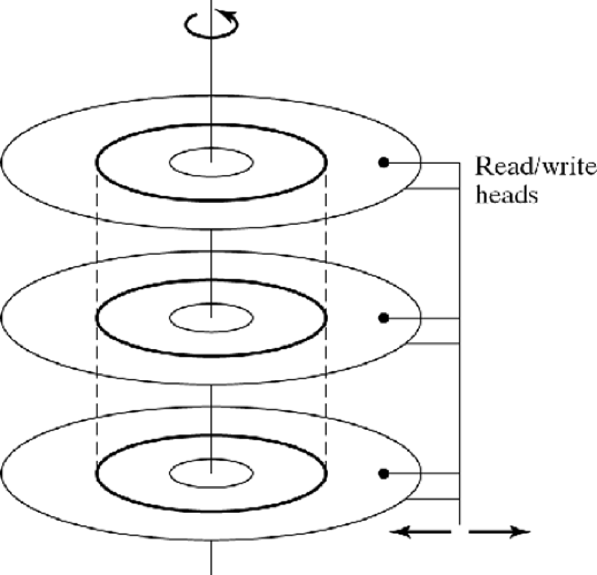
\includegraphics[width=0.5\linewidth]{m3/diskTrackView5}
		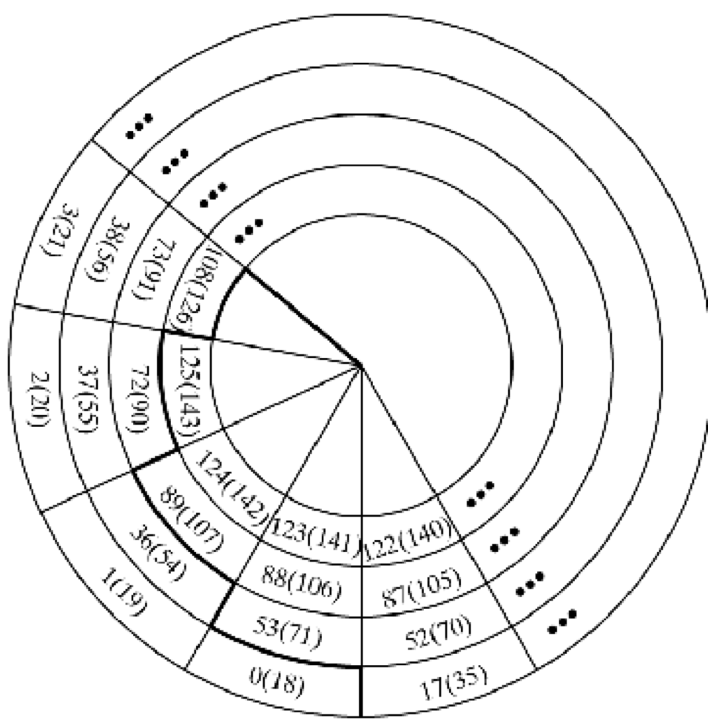
\includegraphics[width=0.5\linewidth]{m3/diskTrackView6}
	\end{minipage}
	
	\textbf{Critical issue: data transfer rates of disks}
	\begin{myitemize}
		\item \textbf{Sustained} rate: continuous data delivery
		\item \textbf{Peek} rate: : transfer once read/write head is in place; depends on rotation speed and data density
	\end{myitemize}
\end{definition}

\begin{example}{Transfer rate calculation:}
	7200 rpm, 100 sectors/track, 512 bytes/sector
	\begin{myitemize}
		\item What is the \textbf{peak} transfer rate?
		\[\frac{7200}{60} \times 100 \times 512 \text{byte/s} \]
		\item What is the \textbf{sustained} transfer rate? - Depends on file organization
	\end{myitemize}
\end{example}

\begin{definition}{\textbf{I/O programming} - access the I/O devices}
	\begin{myitemize}
		\item \textbf{Polling} (You with a broken ringer)
		
		\begin{minipage}{0.48\linewidth}
			\begin{myitemize}
			\item Consider a process that prints “ABCDEFGH” on the printer: The OS then copies character by character onto the printer’s latch, and the printer prints it out.
			\begin{myenumerate}
				\item Copy the first character and advance the buffer’s pointer. 
				\item Check that the printer is ready for the next character. If not, wait. This is called ``busy-waiting'' or ``polling''.
				\item Copy the next character. Repeat until buffer is empty.
			\end{myenumerate}
		\end{myitemize}
		\end{minipage}\hspace{2mm}
		\begin{minipage}{0.48\linewidth}
				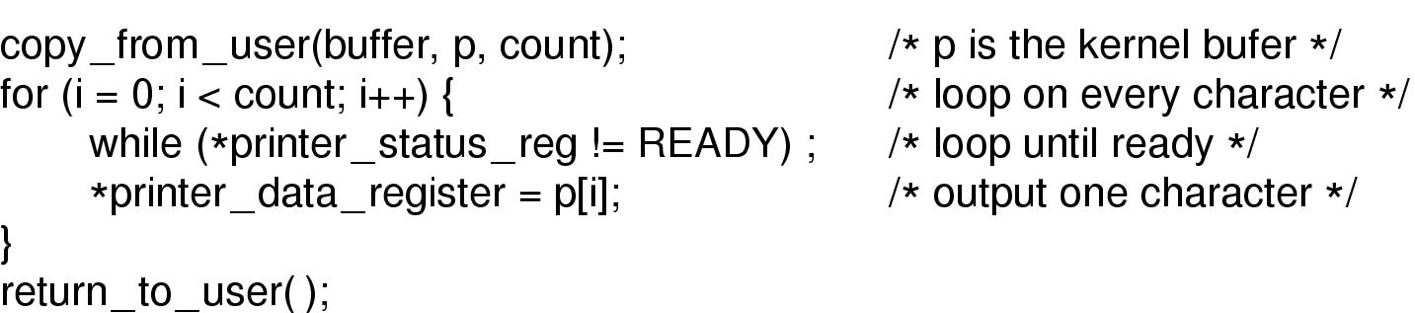
\includegraphics[width=\linewidth]{m3/polling}
				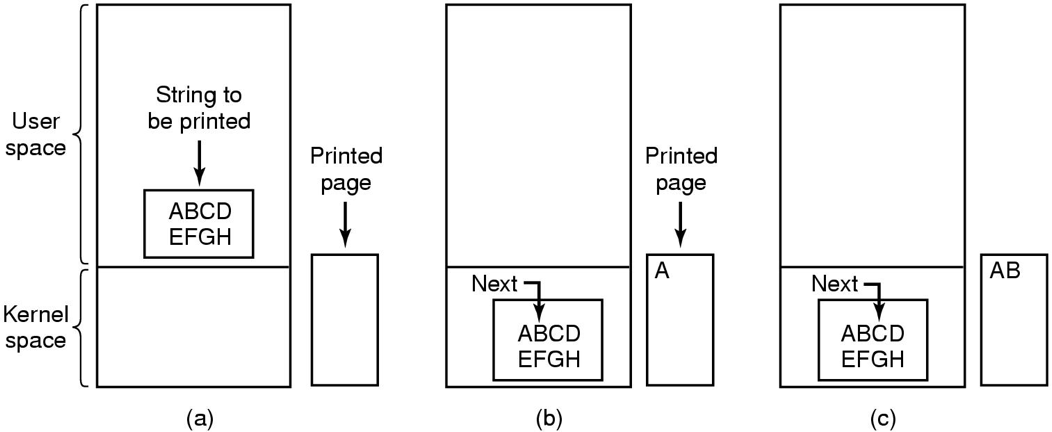
\includegraphics[width=\linewidth]{m3/polling1}
		\end{minipage}
		
		\textbf{Issue}: It takes perhaps 10ms to print a character. During this time, the CPU will be busy-waiting until the printer is done printing. On a 3.2 GHz processor this is equivalent to wasting 320,000,000 instructions! Extremely inefficient use of CPU as most polls are likely to fail. On the other hand not polling risks losing data. 


		\item \textbf{Interrupt-driven I/O} (You with a fully functioning phone)

		\begin{minipage}{0.35\linewidth}
		\begin{myitemize}
			\item After the string is copied, the OS will send a character to the printer, then switch to a task.
			\item When the printer is done, it will interrupt the CPU by asserting one of the “interrupt request” (IRQ) lines on the CPU.
			\item \textbf{Comment}: Some overhead when the hardware is ready, but much less than with polling.
		\end{myitemize}
		\end{minipage}\hspace{5mm}
		\begin{minipage}{0.6\linewidth}
			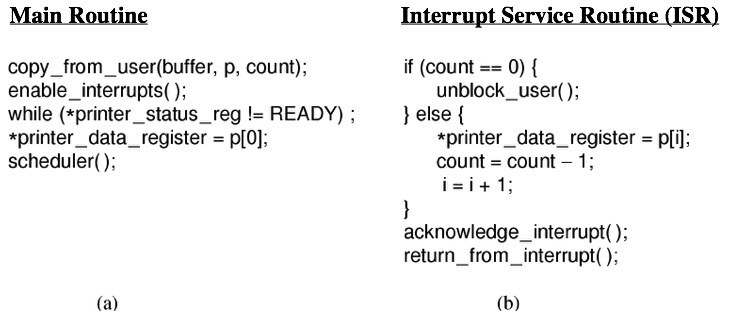
\includegraphics[width=\linewidth]{m3/InterruptIO}
		\end{minipage}
		
		\item \textbf{Direct memory access} (You have an answering machine)
		\begin{myitemize}
			\item \textbf{Driver (CPU) operation to input sequence of bytes:}
			\begin{tcolorbox}
			
				write\_reg(mm\_buf, m);     // give parameters
			
			write\_reg(count, n);
			
			write\_reg(opcode, read);  // start op
			
			block to wait for interrupt;

			\end{tcolorbox}
						\begin{myitemize}
				\item Writing opcode triggers DMA controller
				\item DMA controller issues interrupt after n chars in memory
			\end{myitemize}
			\item \textbf{Cycle Stealing}: 
			\begin{myitemize}
				\item DMA controller competes with CPU for memory access 
				\item generally not a problem because: 1. Memory reference would have occurred anyway; 2. CPU is frequently referencing data in registers or cache, bypassing main memory.
			\end{myitemize}
		\end{myitemize}
	\end{myitemize}
\end{definition}

\begin{definition}{\textbf{Device Management}}
	\begin{myitemize}
		\item \textbf{Disk Scheduling}: Requests for different blocks arrive concurrently from different processes
		\item Minimize \textbf{rotational delay}: re-order requests to blocks on each track to access in one rotation
		\item Minimize \textbf{seek time}: Conflicting goals: Minimize total travel distance; Guarantee fairness
	\end{myitemize}
\end{definition}

\begin{algoalgorithm}{\textbf{Device Management}}

	\begin{minipage}{0.55\linewidth}
		\begin{myitemize}
		\item \textbf{FIFO}: requests are processed in the order of arrival: simple, fair, but inefficient
		\item \textbf{SSTF} (Shortest Seek Time First): most efficient but prone to starvation
		\begin{myitemize}
			\item always go to the track that’s nearest to the current positions
		\end{myitemize} 
		\item \textbf{Scan} (Elevator): fair, acceptable performance
		\begin{myitemize}
			\item maintain a direction of travel
			\item always proceed to the nearest track in the current direction of travel
			\item if there is no request in the current direction, reverse direction
		\end{myitemize}
	\end{myitemize}
	\end{minipage}\hspace{5mm}
	\begin{minipage}{0.4\linewidth}
	
		\textbf{Example}: assume moving from 0 to 5; then 12,4,7 arrive
		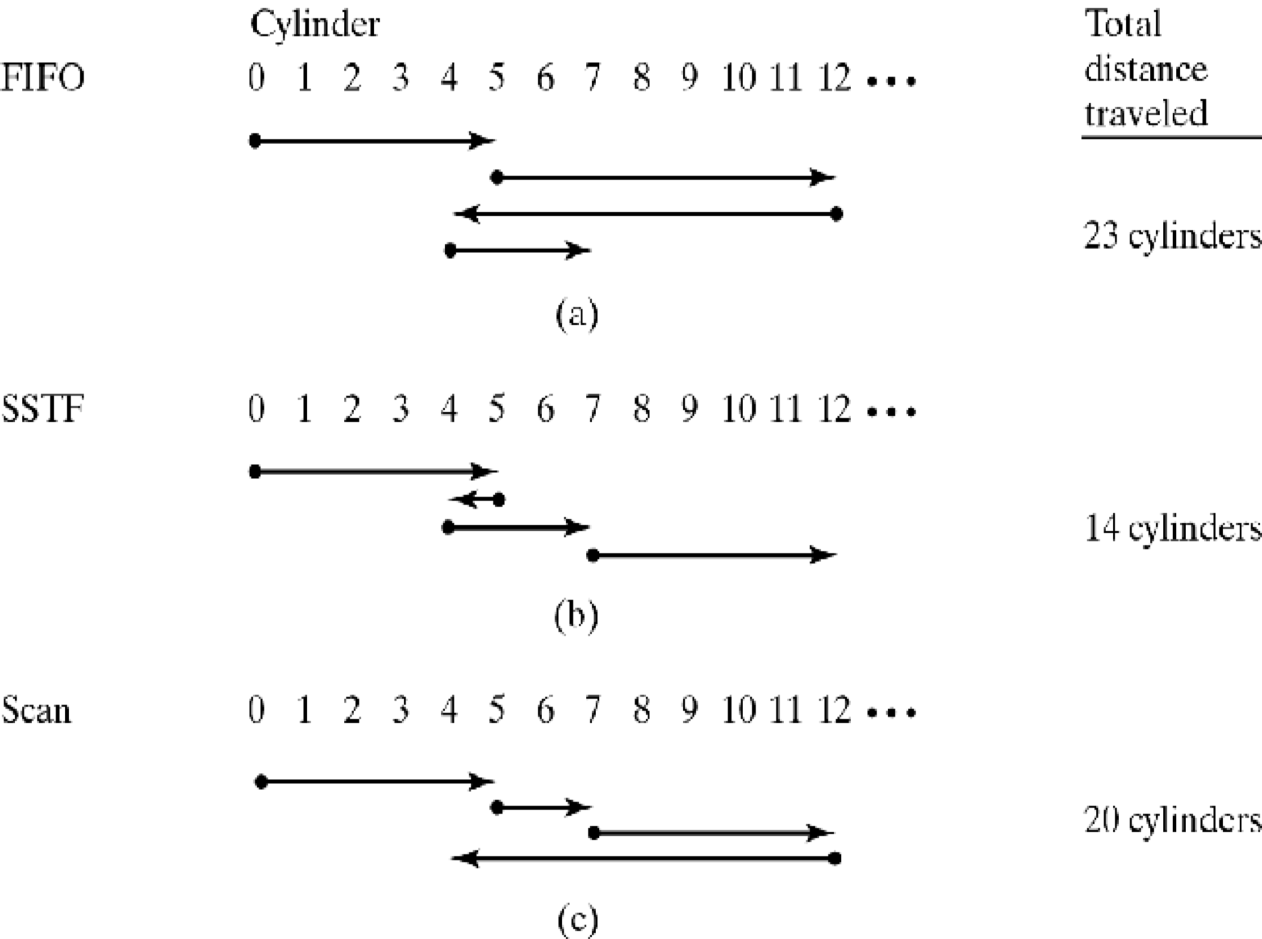
\includegraphics[width=\linewidth]{m3/deviceManagementAlgo}
	\end{minipage}
	
\end{algoalgorithm}

\begin{remark}{\textbf{block size trade off}}
	Larger block sizes means fewer blocks that the OS needs to manage, less overhead. Disadvantage is that there will be greater wastage within each block (internal fragmentation)
\end{remark}

\begin{method}{\textbf{Disk access time calculation}} Time is takes to read one block of data:

\begin{myenumerate}
	\item \textbf{Switch time}: This is the time it takes for the drive to choose the correct side of the correct platter. (can be negligible)
	\item \textbf{Seek time}: This is the time it takes a drive's arm to move to the correct track.
	\item \textbf{Rotational delay}: This is the time it takes for the correct block to move underneath the head. Conventionally, taken to be $\frac{T_r}{2}$, where $T_r$ is the time for one revolution.
	\item \textbf{Transfer delay}: This is the time taken to actually transfer the block. If the disk can transfer M bytes per second and a block is B bytes long, then this time is $\frac{B}{M}$.
\end{myenumerate}

\begin{myitemize}
	\item \textbf{Peak data transfer rate}: The drive cannot be transferring more in one second than the amount of data in one track, multiplied by the number of times that track goes past the head per second
	
	\[ \text{Blocks / Track} = 16, \text{Bytes / Block} = 32768 \]
	\[\text{Bytes / Track} = 16 \times 32768=524288 \text{ bytes},  7200rpm=120rps \]
	\[\text{peak throughput}= 120 \times 524288= 62.9 \text{Megabytes/Sec} (1 \text{megabyte/sec} = 10^6 \text{bytes/sec}) \]
	
	\item \textbf{Time taken on average to read one block of data}:
	\[ \text{Average disk read time =  switching time+seek time+rotational delay+transfer time}\]
	\[\text{rotational delay}=\frac{1}{2} \times \frac{1}{7200/60}=0.0042s \]
	\[\text{Data through put} = 50 \text{ megabits per second} \]
	\[\text{data transfer time}=32768\times 8 / (50,000,000)= 0.0052s = 5.2ms \]
	\textbf{Note}: For storage we conventionally use 1KB = 1024 bytes, not 1000 bytes. However we use 1KB = 1000 bytes for throughput.
\end{myitemize}

\end{method}

\begin{remark}{\textbf{Why interrupts have overheads?}}
	Overheads involved include detecting the interrupt, consulting the vector table to get the interrupt handler address, pushing the current PC to the stack, switching to kernel mode, and vectoring to the interrupt handler and switching back to user mode.
\end{remark}

\begin{example}{\textbf{Compare different I/O Programming methods}}

	\textbf{Question}: Printing 250 characters, how many cycles are wasted on polling?
	
	\textbf{Assumption}: Assuming the printer is currently free, (polling) time for the first character should be negligible. Almost all CPUs can execute at least 1 instruction per cycle
	
	\begin{myitemize}
		\item \textbf{Polling}: For subsequent 249 characters, there is a 10ms poll time between characters. Each clock cycle is 10ns, so this corresponds to approximately 1,000,000 clock cycles per poll, or total of about 249,000,000 cycles to print the entire 250 characters.
		\item \textbf{Interrupt Driven}: For subsequent 249 characters we have total 300ns interrupt time, = 74,700 ns. Each clock cycle is 10ns, so this is equal to 7,470 clock cyles, a great reduction from the original 249,000,000 cycles.
		\item \textbf{DMA}: Total time taken = setup time + end of transfer interrupt processing time = 700ns. This is equal to 70 instructions.
	\end{myitemize}
\end{example}



% $$$$$$$$$$$$$$$$$$$$$$$$$$$$$$$$$$ %
\end{document}